\chapter{Ordenamiento}

\index{ordenamiento}

El \key{ordenamiento}
es un problema fundamental en el diseño de algoritmos.
Muchos algoritmos eficientes
usan el ordenamiento como una subrutina,
ya que a menudo es más fácil procesar
datos si los elementos están en orden.

Por ejemplo, el problema que pregunta "¿un arreglo contiene
dos elementos iguales?" es fácil de resolver usando ordenamiento.
Si el arreglo contiene dos elementos iguales,
estarán uno al lado del otro después de ordenar,
así que es fácil encontrarlos.
Otro problema que pregunta "¿cuál es el elemento más frecuente
en un arreglo?" se puede resolver de manera similar.

Hay muchos algoritmos de ordenamiento, y también son
buenos ejemplos de cómo aplicar
diferentes técnicas de diseño de algoritmos.
Los algoritmos generales de ordenamiento eficientes
funcionan en tiempo $O(n \log n)$,
y muchos algoritmos que utilizan ordenamiento
como una subrutina también
tienen esta complejidad de tiempo.

\section{Teoría del ordenamiento}

El problema básico en el ordenamiento es el siguiente:
\begin{framed}
    \noindent
    Dado un arreglo que contiene $n$ elementos,
    tu tarea es ordenar los elementos
    en orden ascendente.
\end{framed}
\noindent
Por ejemplo, el arreglo
\begin{center}
    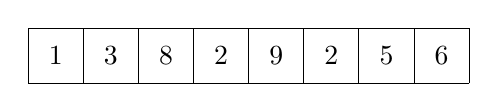
\begin{tikzpicture}[scale=0.7]
        \draw (0,0) grid (8,1);
        \node at (0.5,0.5) {$1$};
        \node at (1.5,0.5) {$3$};
        \node at (2.5,0.5) {$8$};
        \node at (3.5,0.5) {$2$};
        \node at (4.5,0.5) {$9$};
        \node at (5.5,0.5) {$2$};
        \node at (6.5,0.5) {$5$};
        \node at (7.5,0.5) {$6$};
    \end{tikzpicture}
\end{center}
será así después de ordenar:
\begin{center}
    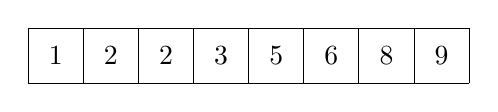
\begin{tikzpicture}[scale=0.7]
        \draw (0,0) grid (8,1);
        \node at (0.5,0.5) {$1$};
        \node at (1.5,0.5) {$2$};
        \node at (2.5,0.5) {$2$};
        \node at (3.5,0.5) {$3$};
        \node at (4.5,0.5) {$5$};
        \node at (5.5,0.5) {$6$};
        \node at (6.5,0.5) {$8$};
        \node at (7.5,0.5) {$9$};
    \end{tikzpicture}
\end{center}

\subsubsection{Algoritmos $O(n^2)$}

\index{ordenamiento burbuja}

Los algoritmos simples para ordenar un arreglo
funcionan en tiempo $O(n^2)$.
Estos algoritmos son cortos y generalmente
consisten en dos bucles anidados.
Un famoso algoritmo de ordenamiento en tiempo $O(n^2)$
es el \key{ordenamiento burbuja}, donde los elementos
``burbujean'' en el arreglo según sus valores.

El ordenamiento burbuja consta de $n$ rondas.
En cada ronda, el algoritmo itera a través
de los elementos del arreglo.
Siempre que se encuentran dos elementos consecutivos
que no están en el orden correcto,
el algoritmo los intercambia.
El algoritmo se puede implementar de la siguiente manera:
\begin{lstlisting}
for (int i = 0; i < n; i++) {
    for (int j = 0; j < n - 1; j++) {
        if (arreglo[j] > arreglo[j+1]) {
            swap(arreglo[j], arreglo[j+1]);
        }
    }
}
\end{lstlisting}

Después de la primera ronda del algoritmo,
el elemento más grande estará en la posición correcta,
y en general, después de $k$ rondas, los $k$ elementos más grandes
estarán en las posiciones correctas.
Por lo tanto, después de $n$ rondas, todo el arreglo
estará ordenado.

Por ejemplo, en el arreglo

\begin{center}
    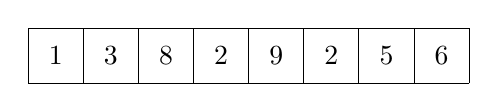
\begin{tikzpicture}[scale=0.7]
        \draw (0,0) grid (8,1);

        \node at (0.5,0.5) {$1$};
        \node at (1.5,0.5) {$3$};
        \node at (2.5,0.5) {$8$};
        \node at (3.5,0.5) {$2$};
        \node at (4.5,0.5) {$9$};
        \node at (5.5,0.5) {$2$};
        \node at (6.5,0.5) {$5$};
        \node at (7.5,0.5) {$6$};
    \end{tikzpicture}
\end{center}

\noindent
la primera ronda de bubble sort intercambia elementos así:

\begin{center}
    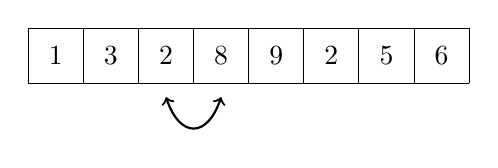
\begin{tikzpicture}[scale=0.7]
        \draw (0,0) grid (8,1);
        \node at (0.5,0.5) {$1$};
        \node at (1.5,0.5) {$3$};
        \node at (2.5,0.5) {$2$};
        \node at (3.5,0.5) {$8$};
        \node at (4.5,0.5) {$9$};
        \node at (5.5,0.5) {$2$};
        \node at (6.5,0.5) {$5$};
        \node at (7.5,0.5) {$6$};

        \draw[thick,<->] (3.5,-0.25) .. controls (3.25,-1.00) and (2.75,-1.00) .. (2.5,-0.25);
    \end{tikzpicture}
\end{center}

\begin{center}
    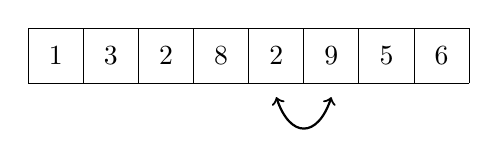
\begin{tikzpicture}[scale=0.7]
        \draw (0,0) grid (8,1);
        \node at (0.5,0.5) {$1$};
        \node at (1.5,0.5) {$3$};
        \node at (2.5,0.5) {$2$};
        \node at (3.5,0.5) {$8$};
        \node at (4.5,0.5) {$2$};
        \node at (5.5,0.5) {$9$};
        \node at (6.5,0.5) {$5$};
        \node at (7.5,0.5) {$6$};

        \draw[thick,<->] (5.5,-0.25) .. controls (5.25,-1.00) and (4.75,-1.00) .. (4.5,-0.25);
    \end{tikzpicture}
\end{center}

\begin{center}
    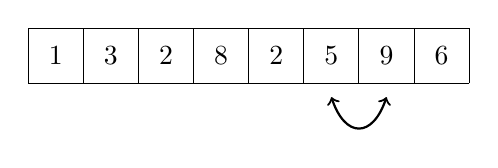
\begin{tikzpicture}[scale=0.7]
        \draw (0,0) grid (8,1);
        \node at (0.5,0.5) {$1$};
        \node at (1.5,0.5) {$3$};
        \node at (2.5,0.5) {$2$};
        \node at (3.5,0.5) {$8$};
        \node at (4.5,0.5) {$2$};
        \node at (5.5,0.5) {$5$};
        \node at (6.5,0.5) {$9$};
        \node at (7.5,0.5) {$6$};

        \draw[thick,<->] (6.5,-0.25) .. controls (6.25,-1.00) and (5.75,-1.00) .. (5.5,-0.25);
    \end{tikzpicture}
\end{center}

\begin{center}
    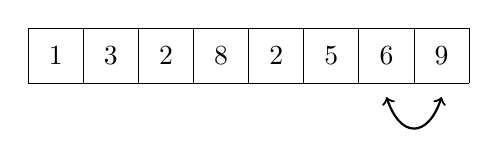
\begin{tikzpicture}[scale=0.7]
        \draw (0,0) grid (8,1);
        \node at (0.5,0.5) {$1$};
        \node at (1.5,0.5) {$3$};
        \node at (2.5,0.5) {$2$};
        \node at (3.5,0.5) {$8$};
        \node at (4.5,0.5) {$2$};
        \node at (5.5,0.5) {$5$};
        \node at (6.5,0.5) {$6$};
        \node at (7.5,0.5) {$9$};

        \draw[thick,<->] (7.5,-0.25) .. controls (7.25,-1.00) and (6.75,-1.00) .. (6.5,-0.25);
    \end{tikzpicture}
\end{center}

\subsubsection{Inversiones}

\index{inversión}

El ordenamiento burbuja es un ejemplo de un algoritmo de ordenamiento
que siempre intercambia elementos \emph{consecutivos}
en el arreglo.
Resulta que la complejidad temporal
de tal algoritmo es \emph{siempre}
al menos $O(n^2)$, porque en el peor caso,
se requieren $O(n^2)$ intercambios para ordenar el arreglo.

\pagebreak Un concepto útil al analizar algoritmos de ordenamiento
es una \key{inversión}:
un par de elementos del arreglo
$(\texttt{arreglo}[a], \texttt{arreglo}[b])$ tal que
$a<b$ y $\texttt{arreglo}[a]>\texttt{arreglo}[b]$,
es decir, los elementos están en el orden incorrecto.
Por ejemplo, el arreglo
\begin{center}
    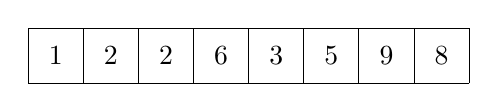
\begin{tikzpicture}[scale=0.7]
        \draw (0,0) grid (8,1);
        \node at (0.5,0.5) {$1$};
        \node at (1.5,0.5) {$2$};
        \node at (2.5,0.5) {$2$};
        \node at (3.5,0.5) {$6$};
        \node at (4.5,0.5) {$3$};
        \node at (5.5,0.5) {$5$};
        \node at (6.5,0.5) {$9$};
        \node at (7.5,0.5) {$8$};
    \end{tikzpicture}
\end{center}
tiene tres inversiones: $(6,3)$, $(6,5)$ y $(9,8)$.
El número de inversiones indica
cuánto trabajo se necesita para ordenar el arreglo.
Un arreglo está completamente ordenado cuando
no hay inversiones.
Por otro lado, si los elementos del arreglo
están en orden inverso,
el número de inversiones es el mayor posible:
\[1+2+\cdots+(n-1)=\frac{n(n-1)}{2} = O(n^2)\]

Intercambiar un par de elementos consecutivos que están
en el orden incorrecto elimina exactamente una inversión
del arreglo.
Por lo tanto, si un algoritmo de ordenamiento solo puede
intercambiar elementos consecutivos, cada intercambio elimina
como máximo una inversión, y la complejidad en tiempo
del algoritmo es al menos $O(n^2)$.

\subsubsection{Algoritmos en $O(n \log n)$}

\index{ordenamiento por mezcla}

Es posible ordenar un arreglo de manera eficiente
en tiempo $O(n \log n)$ utilizando algoritmos
que no se limitan a intercambiar elementos consecutivos.
Un algoritmo de este tipo es el \key{ordenamiento por mezcla}
\footnote{Según \cite{knu983}, el ordenamiento por mezcla fue
    inventado por J. von Neumann en 1945.} (\textit{merge sort}),
que se basa en la recursión.

El ordenamiento por mezcla ordena un subarreglo
\texttt{arreglo}$[a \ldots b]$ de la siguiente manera:

\begin{enumerate}
    \item Si $a=b$, no hacer nada, porque el subarreglo ya está ordenado.
    \item Calcular la posición del elemento medio: $k=\lfloor \frac{a+b}{2} \rfloor$.
    \item Ordenar recursivamente el subarreglo izquierdo \texttt{arreglo}$[a \ldots k]$.
    \item Ordenar recursivamente el subarreglo derecho \texttt{arreglo}$[k+1 \ldots b]$.
    \item \emph{Mezclar} los subarreglos ordenados \texttt{arreglo}$[a \ldots k]$ y
          \texttt{arreglo}$[k+1 \ldots b]$ en un subarreglo ordenado
          \texttt{arreglo}$[a \ldots b]$.
\end{enumerate}

El ordenamiento por mezcla es un algoritmo eficiente, ya que
reduce a la mitad el tamaño del subarreglo en cada paso.
La recursión consta de $O(\log n)$ niveles,
y procesar cada nivel toma tiempo $O(n)$.
Mezclar los subarreglos \texttt{arreglo}$[a \ldots k]$ y
\texttt{arreglo}$[k+1 \ldots b]$
es posible en tiempo lineal, porque ya están ordenados.

Por ejemplo, considera ordenar el siguiente arreglo:
\begin{center}
    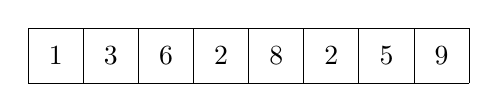
\begin{tikzpicture}[scale=0.7]
        \draw (0,0) grid (8,1);
        \node at (0.5,0.5) {$1$};
        \node at (1.5,0.5) {$3$};
        \node at (2.5,0.5) {$6$};
        \node at (3.5,0.5) {$2$};
        \node at (4.5,0.5) {$8$};
        \node at (5.5,0.5) {$2$};
        \node at (6.5,0.5) {$5$};
        \node at (7.5,0.5) {$9$};
    \end{tikzpicture}
\end{center}

El arreglo se dividirá en dos subarreglos
de la siguiente manera:
\begin{center}
    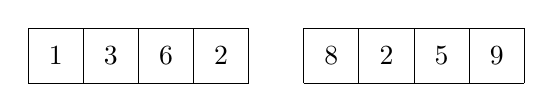
\begin{tikzpicture}[scale=0.7]
        \draw (0,0) grid (4,1);
        \draw (5,0) grid (9,1);

        \node at (0.5,0.5) {$1$};
        \node at (1.5,0.5) {$3$};
        \node at (2.5,0.5) {$6$};
        \node at (3.5,0.5) {$2$};

        \node at (5.5,0.5) {$8$};
        \node at (6.5,0.5) {$2$};
        \node at (7.5,0.5) {$5$};
        \node at (8.5,0.5) {$9$};
    \end{tikzpicture}
\end{center}

Luego, los subarreglos se ordenarán recursivamente
de la siguiente manera:
\begin{center}
    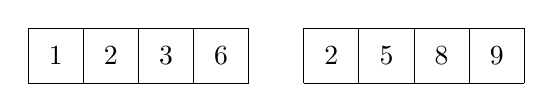
\begin{tikzpicture}[scale=0.7]
        \draw (0,0) grid (4,1);
        \draw (5,0) grid (9,1);

        \node at (0.5,0.5) {$1$};
        \node at (1.5,0.5) {$2$};
        \node at (2.5,0.5) {$3$};
        \node at (3.5,0.5) {$6$};

        \node at (5.5,0.5) {$2$};
        \node at (6.5,0.5) {$5$};
        \node at (7.5,0.5) {$8$};
        \node at (8.5,0.5) {$9$};
    \end{tikzpicture}
\end{center}

Finalmente, estos se combinan para crear el arreglo ordenado final:
\begin{center}
    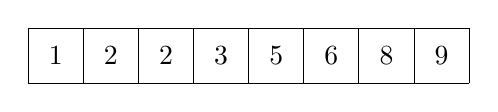
\begin{tikzpicture}[scale=0.7]
        \draw (0,0) grid (8,1);
        \node at (0.5,0.5) {$1$};
        \node at (1.5,0.5) {$2$};
        \node at (2.5,0.5) {$2$};
        \node at (3.5,0.5) {$3$};
        \node at (4.5,0.5) {$5$};
        \node at (5.5,0.5) {$6$};
        \node at (6.5,0.5) {$8$};
        \node at (7.5,0.5) {$9$};
    \end{tikzpicture}
\end{center}

\subsubsection{Cota inferior de ordenamiento}

¿Es posible ordenar un arreglo más rápido
que en tiempo $O(n \log n)$?
Resulta que esto \emph{no} es posible
cuando nos limitamos a algoritmos de ordenamiento
que se basan en comparar elementos del arreglo.

La cota inferior para la complejidad del tiempo
se puede demostrar considerando el ordenamiento
como un proceso en el que cada comparación de dos elementos
proporciona más información sobre el contenido del arreglo.
El proceso crea el siguiente árbol:

\begin{center}
    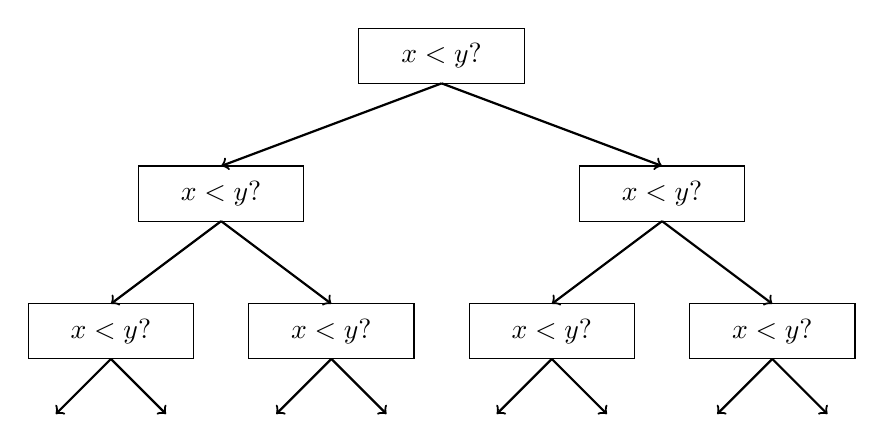
\begin{tikzpicture}[scale=0.7]
        \draw (0,0) rectangle (3,1);
        \node at (1.5,0.5) {$x < y?$};

        \draw[thick,->] (1.5,0) -- (-2.5,-1.5);
        \draw[thick,->] (1.5,0) -- (5.5,-1.5);

        \draw (-4,-2.5) rectangle (-1,-1.5);
        \draw (4,-2.5) rectangle (7,-1.5);
        \node at (-2.5,-2) {$x < y?$};
        \node at (5.5,-2) {$x < y?$};

        \draw[thick,->] (-2.5,-2.5) -- (-4.5,-4);
        \draw[thick,->] (-2.5,-2.5) -- (-0.5,-4);
        \draw[thick,->] (5.5,-2.5) -- (3.5,-4);
        \draw[thick,->] (5.5,-2.5) -- (7.5,-4);

        \draw (-6,-5) rectangle (-3,-4);
        \draw (-2,-5) rectangle (1,-4);
        \draw (2,-5) rectangle (5,-4);
        \draw (6,-5) rectangle (9,-4);
        \node at (-4.5,-4.5) {$x < y?$};
        \node at (-0.5,-4.5) {$x < y?$};
        \node at (3.5,-4.5) {$x < y?$};
        \node at (7.5,-4.5) {$x < y?$};

        \draw[thick,->] (-4.5,-5) -- (-5.5,-6);
        \draw[thick,->] (-4.5,-5) -- (-3.5,-6);
        \draw[thick,->] (-0.5,-5) -- (0.5,-6);
        \draw[thick,->] (-0.5,-5) -- (-1.5,-6);
        \draw[thick,->] (3.5,-5) -- (2.5,-6);
        \draw[thick,->] (3.5,-5) -- (4.5,-6);
        \draw[thick,->] (7.5,-5) -- (6.5,-6);
        \draw[thick,->] (7.5,-5) -- (8.5,-6);
    \end{tikzpicture}
\end{center}

Aquí ``$x<y?$'' significa que algunos elementos
$x$ e $y$ son comparados.
Si $x<y$, el proceso continúa a la izquierda,
y en caso contrario a la derecha.
Los resultados del proceso son las posibles
maneras de ordenar el arreglo, un total de $n!$ maneras.
Por esta razón, la altura del árbol
debe ser al menos
\[ \log_2(n!) = \log_2(1)+\log_2(2)+\cdots+\log_2(n).\]
Obtenemos una cota inferior para esta suma
al elegir los últimos $n/2$ elementos y
cambiar el valor de cada elemento a $\log_2(n/2)$.
Esto produce una estimación
\[ \log_2(n!) \ge (n/2) \cdot \log_2(n/2),\]
por lo que la altura del árbol y el mínimo
número posible de pasos en un algoritmo de ordenamiento
en el peor caso
es al menos $n \log n$.

\subsubsection{Ordenamiento por conteo}

\index{ordenamiento por conteo}

La cota inferior $n \log n$ no se aplica a
algoritmos que no comparan elementos del arreglo
sino que utilizan alguna otra información.
Un ejemplo de tal algoritmo es el
\key{ordenamiento por conteo}, que ordena un arreglo en
$O(n)$ suponiendo que cada elemento en el arreglo
es un entero entre $0 \ldots c$ y $c=O(n)$.

El algoritmo crea un arreglo de \emph{registro},
cuyos índices son elementos del arreglo original.
El algoritmo itera a través del arreglo original
y calcula cuántas veces aparece cada elemento
en el arreglo.

Por ejemplo, el arreglo
\begin{center}
    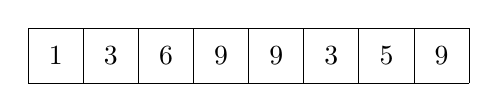
\begin{tikzpicture}[scale=0.7]
        \draw (0,0) grid (8,1);
        \node at (0.5,0.5) {$1$};
        \node at (1.5,0.5) {$3$};
        \node at (2.5,0.5) {$6$};
        \node at (3.5,0.5) {$9$};
        \node at (4.5,0.5) {$9$};
        \node at (5.5,0.5) {$3$};
        \node at (6.5,0.5) {$5$};
        \node at (7.5,0.5) {$9$};
    \end{tikzpicture}
\end{center}
corresponde al siguiente arreglo de registro:
\begin{center}
    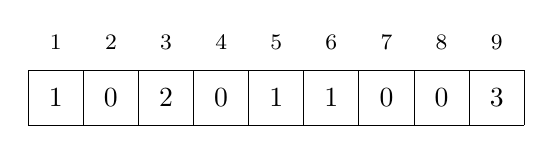
\begin{tikzpicture}[scale=0.7]
        \draw (0,0) grid (9,1);
        \node at (0.5,0.5) {$1$};
        \node at (1.5,0.5) {$0$};
        \node at (2.5,0.5) {$2$};
        \node at (3.5,0.5) {$0$};
        \node at (4.5,0.5) {$1$};
        \node at (5.5,0.5) {$1$};
        \node at (6.5,0.5) {$0$};
        \node at (7.5,0.5) {$0$};
        \node at (8.5,0.5) {$3$};

        \footnotesize

        \node at (0.5,1.5) {$1$};
        \node at (1.5,1.5) {$2$};
        \node at (2.5,1.5) {$3$};
        \node at (3.5,1.5) {$4$};
        \node at (4.5,1.5) {$5$};
        \node at (5.5,1.5) {$6$};
        \node at (6.5,1.5) {$7$};
        \node at (7.5,1.5) {$8$};
        \node at (8.5,1.5) {$9$};
    \end{tikzpicture}
\end{center}

Por ejemplo, el valor en la posición 3
en el arreglo de registro es 2,
porque el elemento 3 aparece 2 veces
en el arreglo original.

La construcción del arreglo de registro
toma un tiempo de $O(n)$. Después de esto, el arreglo ordenado
se puede crear en tiempo $O(n)$ porque
el número de ocurrencias de cada elemento se puede obtener
del arreglo de registro.
Por lo tanto, la complejidad total en tiempo del
ordenamiento por conteo es $O(n)$.

El ordenamiento por conteo es un algoritmo muy eficiente
pero solo se puede usar cuando la constante $c$
es lo suficientemente pequeña, de modo que los elementos del arreglo puedan
usarse como índices en el arreglo de registro.

\section{Ordenamiento en C++}

\index{sort@\texttt{sort}}

Casi nunca es una buena idea usar
un algoritmo de ordenamiento casero
en un concurso, porque hay buenas
implementaciones disponibles en cada lenguaje de programación.
Por ejemplo, la biblioteca estándar de C++ contiene
la función \texttt{sort} que se puede utilizar fácilmente para
ordenar arreglos y otras estructuras de datos.

Hay muchos beneficios al usar una función de biblioteca.
En primer lugar, ahorra tiempo porque no hay necesidad de
implementar la función.
En segundo lugar, la implementación de la biblioteca es
ciertamente correcta y eficiente: no es probable
que una función casera sea mejor.

En esta sección veremos cómo utilizar la
función \texttt{sort} de C++.
El siguiente código ordena
un vector en orden creciente:
\begin{lstlisting}
vector<int> v = {4, 2, 5, 3, 5, 8, 3};
sort(v.begin(), v.end());
\end{lstlisting}
Después del ordenamiento, el contenido del
vector será
$[2,3,3,4,5,5,8]$.
El orden de clasificación predeterminado es creciente,
pero un orden inverso es posible de la siguiente manera:
\begin{lstlisting}
sort(v.rbegin(), v.rend());
\end{lstlisting}

Se puede ordenar un arreglo ordinario de la siguiente manera:
\begin{lstlisting}
int n = 7; // tamaño del arreglo
int a[] = {4, 2, 5, 3, 5, 8, 3};
sort(a, a + n);
\end{lstlisting}

\noindent
El siguiente código ordena la cadena \texttt{s}:
\begin{lstlisting}
string s = "monito";
sort(s.begin(), s.end());
\end{lstlisting}
Ordenar una cadena significa que los caracteres
de la cadena se ordenan.
Por ejemplo, la cadena ``monito'' se convierte en ``imnoot''.

\subsubsection{Operadores de comparación}

\index{operador de comparación}

La función \texttt{sort} requiere que
se defina un \key{operador de comparación} para el tipo de dato
de los elementos a ordenar.
Al ordenar, este operador se utilizará
siempre que sea necesario averiguar el orden de dos elementos.

La mayoría de los tipos de datos en C++ tienen un operador de comparación incorporado,
y los elementos de esos tipos se pueden ordenar automáticamente.
Por ejemplo, los números se ordenan según sus valores
y las cadenas de caracteres se ordenan alfabéticamente.

\index{par@\texttt{pair}}

Los pares (\texttt{pair}) se ordenan principalmente según sus
primeros elementos (\texttt{first}).
Sin embargo, si los primeros elementos de dos pares son iguales,
se ordenan según sus segundos elementos (\texttt{second}):
\begin{lstlisting}
vector<pair<int, int>> v;
v.push_back({1, 5});
v.push_back({2, 3});
v.push_back({1, 2});
sort(v.begin(), v.end());
\end{lstlisting}
Después de esto, el orden de los pares es
$(1,2)$, $(1,5)$ y $(2,3)$.

\index{tuple@\texttt{tuple}}

De manera similar, las tuplas (\texttt{tuple})
se ordenan principalmente por el primer elemento,
secundariamente por el segundo elemento, etc.:\footnote{Cabe mencionar que en algunos compiladores antiguos,
    la función \texttt{make\_tuple} debe utilizarse para crear una tupla en lugar de
    llaves (por ejemplo, \texttt{make\_tuple(2,1,4)} en lugar de \texttt{\{2,1,4\}}).}
\begin{lstlisting}
vector<tuple<int, int, int>> v;
v.push_back({2, 1, 4});
v.push_back({1, 5, 3});
v.push_back({2, 1, 3});
sort(v.begin(), v.end());
\end{lstlisting}
Después de esto, el orden de las tuplas es
$(1, 5, 3)$, $(2, 1, 3)$ y $(2, 1, 4)$.

\subsubsection{Estructuras propias}

\index{struct@\texttt{struct}}

Las estructuras (\texttt{struct}) definidas por el usuario
no tienen un operador de comparación
automáticamente.
El operador debe definirse dentro
del struct como una función
\texttt{operator<},
cuyo parámetro es otro elemento del mismo tipo.
El operador debe devolver \texttt{true}
si el elemento es menor que el parámetro,
y \texttt{false} en caso contrario.

Por ejemplo, el siguiente struct \texttt{P}
contiene las coordenadas \texttt{x} e \texttt{y} de un punto.
El operador de comparación se define de tal manera que
los puntos se ordenan principalmente por la coordenada \texttt{x}
y secundariamente por la coordenada \texttt{y}.

\begin{lstlisting}
struct P {
    int x, y;
    bool operator<(const P &p) {
        if (x != p.x) return x < p.x;
        else return y < p.y;
    }
}
\end{lstlisting}

\subsubsection{Funciones de comparación}

\index{función de comparación}

También es posible proporcionar una
\key{función de comparación} externa a la función \texttt{sort}
como una función de retrollamada (o \textit{callback}).
Por ejemplo, la siguiente función de comparación \texttt{comp}
ordena las cadenas de texto principalmente por longitud y secundariamente
por orden alfabético:

\begin{lstlisting}
bool comp(string a, string b) {
    if (a.size() != b.size()) return a.size() < b.size();
    return a < b;
}
\end{lstlisting}
Ahora un vector de cadenas de texto se puede ordenar de la siguiente manera:
\begin{lstlisting}
sort(v.begin(), v.end(), comp);
\end{lstlisting}

\section{Búsqueda binaria}

\index{búsqueda binaria}

Un método general para buscar un elemento
en un arreglo es usar un bucle \texttt{for}
que itere a través de los elementos del arreglo.
Por ejemplo, el siguiente código busca
un elemento $x$ en un arreglo:

\begin{lstlisting}
for (int i = 0; i < n; i++) {
    if (arreglo[i] == x) {
        // x encontrado en el índice i
    }
}
\end{lstlisting}

La complejidad temporal de este método es $O(n)$,
porque en el peor caso, es necesario verificar
todos los elementos del arreglo.
Si el orden de los elementos es arbitrario,
este también es el mejor método posible, porque
no hay información adicional disponible sobre dónde
en el arreglo deberíamos buscar el elemento $x$.

Sin embargo, si el arreglo está \emph{ordenado},
la situación es diferente.
En este caso, es posible realizar la
búsqueda mucho más rápido, porque el orden de los
elementos en el arreglo guía la búsqueda.
El siguiente algoritmo de \key{búsqueda binaria}
busca eficientemente un elemento en un arreglo ordenado
en tiempo $O(\log n)$.

\subsubsection{Método 1}

La forma habitual de implementar la búsqueda binaria
se asemeja a buscar una palabra en un diccionario.
La búsqueda mantiene una región activa en el arreglo,
que inicialmente contiene todos los elementos del arreglo.
Luego, se realizan una serie de pasos,
cada uno de los cuales divide por la mitad el tamaño de la región.

En cada paso, la búsqueda verifica el elemento central
de la región activa.
Si el elemento central es el elemento objetivo,
la búsqueda termina.
De lo contrario, la búsqueda continúa recursivamente
en la mitad izquierda o derecha de la región,
dependiendo del valor del elemento central.

La idea anterior se puede implementar de la siguiente manera:
\begin{lstlisting}
int a = 0, b = n - 1;
while (a <= b) {
    int k = (a + b) / 2;
    if (arreglo[k] == x) {
        // x encontrado en el índice k
    }
    if (arreglo[k] > x) b = k - 1;
    else a = k + 1;
}
\end{lstlisting}

En esta implementación, la región activa es $a \ldots b$,
y al principio la región es $0 \ldots n-1$.
El algoritmo reduce a la mitad el tamaño de la región en cada paso,
por lo que la complejidad temporal es $O(\log n)$.

\subsubsection{Método 2}

Un método alternativo para implementar la búsqueda binaria
se basa en una forma eficiente de iterar a través de
los elementos del arreglo.
La idea es hacer saltos y disminuir la velocidad
cuando nos acercamos al elemento objetivo.

La búsqueda recorre el arreglo de izquierda a
derecha, y la longitud inicial del salto es $n/2$.
En cada paso, la longitud del salto se dividirá a la mitad:
primero $n/4$, luego $n/8$, $n/16$, etc., hasta
que finalmente la longitud sea 1.
Después de los saltos, sabemos que se ha encontrado el elemento
objetivo o que no aparece en el arreglo.

\newpage
El siguiente código implementa la idea anterior:
\begin{lstlisting}
int k = 0;
for (int b = n / 2; b >= 1; b /= 2) {
    while (k + b < n && arreglo[k + b] <= x) k += b;
}
if (arreglo[k] == x) {
    // x encontrado en el índice k
}
\end{lstlisting}

Durante la búsqueda, la variable $b$
contiene la longitud actual del salto.
La complejidad temporal del algoritmo es $O(\log n)$,
porque el código en el bucle \texttt{while}
se realiza como máximo dos veces para cada longitud de salto.

\subsubsection{Funciones de C++}

El encabezado \texttt{<algorithm>} de la biblioteca estándar
de C++ contiene las siguientes funciones
que se basan en la búsqueda binaria y funcionan en tiempo logarítmico:

\begin{itemize}
    \item \texttt{lower\_bound} devuelve un puntero al
          primer elemento del arreglo cuyo valor es al menos $x$.
    \item \texttt{upper\_bound} devuelve un puntero al
          primer elemento del arreglo cuyo valor es mayor que $x$.
    \item \texttt{equal\_range} devuelve ambos punteros.
\end{itemize}

Las funciones asumen que el arreglo está ordenado.
Si no hay tal elemento, el puntero apunta al
elemento después del último elemento del arreglo.
Por ejemplo, el siguiente código averigua si
un arreglo contiene un elemento con valor $x$:

\begin{lstlisting}
auto k = lower_bound(arreglo, arreglo + n, x) - arreglo;
if (k < n && arreglo[k] == x) // x encontrado en el índice k
\end{lstlisting}

El siguiente código cuenta la cantidad de elementos
cuyo valor es $x$ en un arreglo:

\begin{lstlisting}
auto a = lower_bound(arreglo, arreglo + n, x);
auto b = upper_bound(arreglo, arreglo + n, x);
cout << b - a << "\n";
\end{lstlisting}

Usando \texttt{equal\_range}, el código se vuelve más corto:

\begin{lstlisting}
auto r = equal_range(arreglo, arreglo + n, x);
cout << r.second - r.first << "\n";
\end{lstlisting}

\subsubsection{Encontrar la solución más pequeña}

Un uso importante para la búsqueda binaria es
encontrar la posición en la que el valor de una \emph{función} cambia.
Supongamos que queremos encontrar el valor más pequeño $k$
que es una solución válida para un problema.
Se nos da una función $\texttt{ok}(x)$
que devuelve \texttt{true} si $x$ es una solución válida
y \texttt{false} en caso contrario.
Además, sabemos que $\texttt{ok}(x)$ es \texttt{false}
cuando $x < k$ y \texttt{true} cuando $x \ge k$.
La situación se ve de la siguiente manera:

\begin{center}
    \begin{tabular}{r|rrrrrrrr}
        $x$              & 0              & 1              & $\cdots$      & $k-1$         & $k$      & $k+1$ & $\cdots$ \\
        \hline
        $\texttt{ok}(x)$ & \texttt{false} & \texttt{false}
                         & $\cdots$       & \texttt{false} & \texttt{true} & \texttt{true} & $\cdots$                    \\
    \end{tabular}
\end{center}

\noindent
Ahora, el valor de $k$ se puede encontrar usando búsqueda binaria:

\begin{lstlisting}
int x = -1;
for (int b = z; b >= 1; b /= 2) {
    while (!ok(x + b)) x += b;
}
int k = x + 1;
\end{lstlisting}

La búsqueda encuentra el mayor valor de $x$ para el cual
$\texttt{ok}(x)$ es \texttt{false}.
Por lo tanto, el siguiente valor $k=x+1$
es el valor más pequeño posible para el cual
$\texttt{ok}(k)$ es \texttt{true}.
La longitud del salto inicial $z$ debe ser
suficientemente grande, por ejemplo, algún valor
para el cual sepamos de antemano que $\texttt{ok}(z)$ es \texttt{true}.

El algoritmo llama a la función \texttt{ok}
$O(\log z)$ veces, por lo que la complejidad total del tiempo
depende de la función \texttt{ok}.
Por ejemplo, si la función funciona en tiempo $O(n)$,
la complejidad total del tiempo es $O(n \log z)$.

\subsubsection{Encontrar el valor máximo}

La búsqueda binaria también se puede utilizar para encontrar
el valor máximo de una función que primero aumenta y luego disminuye.
Nuestra tarea es encontrar una posición $k$ tal que

\begin{itemize}
    \item
          $f(x)<f(x+1)$ cuando $x<k$, y
    \item
          $f(x)>f(x+1)$ cuando $x \ge k$.
\end{itemize}

La idea es utilizar la búsqueda binaria
para encontrar el mayor valor de $x$
para el cual $f(x)<f(x+1)$.
Esto implica que $k=x+1$
porque $f(x+1)>f(x+2)$.
El siguiente código implementa la búsqueda:

\begin{lstlisting}
int x = -1;
for (int b = z; b >= 1; b /= 2) {
    while (f(x + b) < f(x + b + 1)) x += b;
}
int k = x + 1;
\end{lstlisting}

Ten en cuenta que a diferencia de la búsqueda binaria ordinaria,
aquí no está permitido que los valores consecutivos
de la función sean iguales, ya que
en este caso, no sería posible saber
cómo continuar la búsqueda.
